% Model 2 visual restriction & accounting chart (replaces wall of inequalities).
% Four resource pillars matching Problem B: Funding, Water, Land & Grid, Labour.
% Build: cd Paper/Figure && pdflatex m2_restrictions.tex
\documentclass[tikz,border=3pt]{standalone}
\usepackage{newtxtext,newtxmath}
\usepackage{amsmath,bm}
\usetikzlibrary{arrows.meta,calc,backgrounds}
% Shared colours for the TikZ schematics; same roles and hex values as
% Code/figures_matlab/paper_style.m (mycolor.space, base #1E5F74).
%   water (P, I, M, W-bar)  teal   | vegetation (V, r, d)  green
%   wind and sand (E, S)    brown  | highlight             orange
%   limits and caps         red dashed
\definecolor{pWater}{HTML}{1E5F74}
\definecolor{pWaterMid}{HTML}{659FB6}
\definecolor{pWaterLight}{HTML}{DCEBF1}
\definecolor{pTeal}{HTML}{00828C}
\definecolor{pVeg}{HTML}{2B633C}
\definecolor{pVegMid}{HTML}{4AC087}
\definecolor{pVegLight}{HTML}{E3F3E8}
\definecolor{pSand}{HTML}{8F7159}
\definecolor{pSandLight}{HTML}{FFEACE}
\definecolor{pAccent}{HTML}{F49431}
\definecolor{pPV}{HTML}{D47216}
\definecolor{pPVLight}{HTML}{FDF1E3}
\definecolor{pPlum}{HTML}{7A437F}
\definecolor{pPlumLight}{HTML}{F2EBF3}
\definecolor{pLimit}{HTML}{D03B3B}
\definecolor{pInk}{HTML}{1F2B33}
\definecolor{pAxis}{HTML}{344A53}
\definecolor{pGrey}{HTML}{97AFB9}
\definecolor{pGreyDark}{HTML}{647B84}
\definecolor{pGrid}{HTML}{E6EBED}

\tikzset{
  pill/.style={rectangle, rounded corners=2.5pt, line width=0.85pt, draw=#1, fill=#1,
    text=white, font=\small\bfseries, align=center, minimum width=2.45cm, minimum height=0.96cm, inner sep=3pt},
  usebox/.style={rectangle, rounded corners=2.5pt, line width=0.75pt, draw=#1, fill=#1!9,
    text=pInk, font=\footnotesize, align=left, text width=6.45cm, minimum height=0.96cm, inner xsep=5pt, inner ysep=3pt},
  capbox/.style={rectangle, rounded corners=2.5pt, line width=0.8pt, draw=pLimit,
    dash pattern=on 3.5pt off 2pt, fill=pLimit!6, text=pInk, font=\footnotesize,
    align=left, text width=5.75cm, minimum height=0.96cm, inner xsep=5pt, inner ysep=3pt},
  leq/.style={font=\normalsize\bfseries, text=pLimit},
  colh/.style={font=\scriptsize\bfseries, text=pGreyDark, anchor=south},
}
\begin{document}
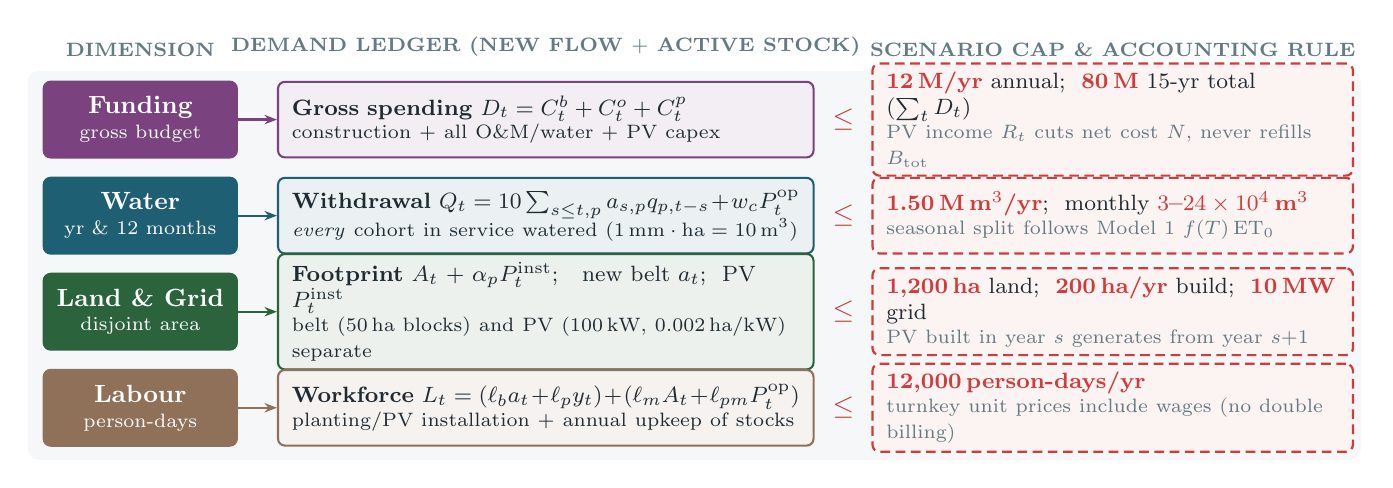
\begin{tikzpicture}
% Column headers
\node[colh] at (1.25, 0.68)  {DIMENSION};
\node[colh] at (6.40, 0.68)  {DEMAND LEDGER (NEW FLOW $+$ ACTIVE STOCK)};
\node[colh] at (13.60, 0.68) {SCENARIO CAP \& ACCOUNTING RULE};

% Row 1: Funding
\node[pill=pPlum]   (p1) at (1.25,  0.00) {Funding\\[-2pt]{\scriptsize\normalfont gross budget}};
\node[usebox=pPlum] (u1) at (6.40,  0.00) {\textbf{Gross spending} $D_t = C_t^b + C_t^o + C_t^p$\\[-1pt]{\scriptsize construction $+$ all O\&M/water $+$ PV capex}};
\node[leq]               at (10.18, 0.00) {$\le$};
\node[capbox]       (c1) at (13.60, 0.00) {{\color{pLimit}\textbf{12\,M/yr}} annual; \ {\color{pLimit}\textbf{80\,M}} 15-yr total ($\sum_t D_t$)\\[-1pt]{\scriptsize\color{pGreyDark}PV income $R_t$ cuts net cost $N$, never refills $B_{\mathrm{tot}}$}};

% Row 2: Water
\node[pill=pWater]   (p2) at (1.25,  -1.22) {Water\\[-2pt]{\scriptsize\normalfont yr \& 12 months}};
\node[usebox=pWater] (u2) at (6.40,  -1.22) {\textbf{Withdrawal} $Q_t = 10\sum_{s\le t,p}a_{s,p}q_{p,t-s} + w_c P_t^{\mathrm{op}}$\\[-1pt]{\scriptsize \emph{every} cohort in service watered ($1\text{\,mm}\cdot\text{ha}=10\text{\,m}^3$)}};
\node[leq]                at (10.18, -1.22) {$\le$};
\node[capbox]        (c2) at (13.60, -1.22) {{\color{pLimit}\textbf{1.50\,M\,m$^3$/yr}}; \ monthly {\color{pLimit}\textbf{$3\text{--}24\times10^4$\,m$^3$}}\\[-1pt]{\scriptsize\color{pGreyDark}seasonal split follows Model~1 $f(T)\,\mathrm{ET}_0$}};

% Row 3: Land & Grid
\node[pill=pVeg]   (p3) at (1.25,  -2.44) {Land \& Grid\\[-2pt]{\scriptsize\normalfont disjoint area}};
\node[usebox=pVeg] (u3) at (6.40,  -2.44) {\textbf{Footprint} $A_t + \alpha_p P_t^{\mathrm{inst}}$;\quad new belt $a_t$; \ PV $P_t^{\mathrm{inst}}$\\[-1pt]{\scriptsize belt ($50$\,ha blocks) and PV ($100$\,kW, $0.002$\,ha/kW) separate}};
\node[leq]              at (10.18, -2.44) {$\le$};
\node[capbox]      (c3) at (13.60, -2.44) {{\color{pLimit}\textbf{1{,}200\,ha}} land; \ {\color{pLimit}\textbf{200\,ha/yr}} build; \ {\color{pLimit}\textbf{10\,MW}} grid\\[-1pt]{\scriptsize\color{pGreyDark}PV built in year $s$ generates from year $s{+}1$}};

% Row 4: Labour
\node[pill=pSand]   (p4) at (1.25,  -3.66) {Labour\\[-2pt]{\scriptsize\normalfont person-days}};
\node[usebox=pSand] (u4) at (6.40,  -3.66) {\textbf{Workforce} $L_t = (\ell_b a_t + \ell_p y_t) + (\ell_m A_t + \ell_{pm} P_t^{\mathrm{op}})$\\[-1pt]{\scriptsize planting/PV installation $+$ annual upkeep of stocks}};
\node[leq]               at (10.18, -3.66) {$\le$};
\node[capbox]       (c4) at (13.60, -3.66) {{\color{pLimit}\textbf{12{,}000\,person-days/yr}}\\[-1pt]{\scriptsize\color{pGreyDark}turnkey unit prices include wages (no double billing)}};

% Clean connectors from pillar badge to demand box
\foreach \k/\col in {1/pPlum, 2/pWater, 3/pVeg, 4/pSand}
  \draw[-{Stealth[length=4.5pt]}, \col, line width=0.8pt] (p\k.east) -- (u\k.west);

% Background frame
\begin{scope}[on background layer]
  \fill[pGrid!40, rounded corners=4pt] (-0.18, 0.62) rectangle (16.75, -4.32);
\end{scope}
\end{tikzpicture}
\end{document}
